% !BIB TS-program = biber
% !BIB program = biber
\documentclass[times]{itmo-student-thesis}

%% Опции пакета:
%% - specification - если есть, генерируется задание, иначе не генерируется
%% - annotation - если есть, генерируется аннотация, иначе не генерируется
%% - times - делает все шрифтом Times New Roman, собирается с помощью xelatex
%% - languages={...} - устанавливает перечень используемых языков. По умолчанию это {english,russian}.
%%                     Последний из языков определяет текст основного документа.

\usepackage{graphicx}
\graphicspath{ {./img/} }

%% Делает запятую в формулах более интеллектуальной, например:
%% $1,5x$ будет читаться как полтора икса, а не один запятая пять иксов.
%% Однако если написать $1, 5x$, то все будет как прежде.
\usepackage{icomma}

%% Один из пакетов, позволяющий делать таблицы на всю ширину текста.
\usepackage{tabularx}

%% Данные пакеты необязательны к использованию в бакалаврских/магистерских
%% Они нужны для иллюстративных целей
%% Начало
\usepackage{tikz}
\usetikzlibrary{arrows}
\usepackage{filecontents}
\begin{filecontents}{master-thesis.bib}

@online{ programmatic-buying,
    title = {Programmatic Buying - Definition and Demarcation},
    url = {https://en.ryte.com/wiki/Programmatic_Buying},
    langid = {english},
    urldate = {2020-05-26}
}

@online{ growth-of-programmatic,
    title = {How is programmatic marketing and digital display advertising defined},
    url = {https://www.smartinsights.com/internet-advertising/internet-advertising-targeting/what-is-programmatic-marketing/},
    langid = {english},
    urldate = {2020-05-26}
}

@online{ ad-server,
    title = {Ad serving},
    url = {https://en.wikipedia.org/wiki/Ad_serving},
    langid = {english},
    urldate = {2020-05-26}
}

@online{ three-tier-architecture,
    title = {Three-tier architecture},
    url = {https://en.wikipedia.org/wiki/Multitier_architecture#Three-tier_architecture},
    langid = {english},
    urldate = {2020-05-26}
}

@online{ data-access-layer,
    title = {Data access layer},
    url = {https://en.wikipedia.org/wiki/Data_access_layer},
    langid = {english},
    urldate = {2020-05-26}
}

@online{ twelve-factor-app,
    title = {The Twelve-Factor App},
    url = {https://12factor.net/},
    langid = {english},
    urldate = {2020-05-26}
}

@online{ mongodb,
    title = {The most popular database for modern apps | MongoDB},
    url = {https://www.mongodb.com/},
    langid = {english},
    urldate = {2020-05-26}
}

@online{ amazon-paapi-docs,
    title = {Product Advertising API 5.0 - documentation},
    url = {https://webservices.amazon.com/paapi5/documentation/},
    langid = {english},
    urldate = {2020-05-26}
}

@online{ amazon-paapi-sdk,
    title = {Product Advertising API 5.0 - Node.js SDK},
    url = {https://webservices.amazon.com/paapi5/documentation/assets/archives/paapi5-nodejs-sdk-example.zip},
    langid = {english},
    urldate = {2020-05-26}
}

@online{ repository-pattern,
    title = {Repository Pattern},
    url = {https://deviq.com/repository-pattern/},
    langid = {english},
    urldate = {2020-05-26}
}

@online{ typescript-lang,
    title = {TypeScript - JavaScript that scales.},
    url = {https://www.typescriptlang.org/},
    langid = {english},
    urldate = {2020-05-26}
}

@online{ contextual-targeting,
    title = {Contextual advertising},
    url = {https://en.wikipedia.org/wiki/Contextual_advertising},
    langid = {english},
    urldate = {2020-05-26}
}

@online{ behavioural-targeting,
    title = {Behavioural targeting},
    url = {https://en.wikipedia.org/wiki/Targeted_advertising#Behavioural_targeting},
    langid = {english},
    urldate = {2020-05-26}
}

@online{ creative-sequencing,
    title = {Creative sequencing},
    url = {https://en.wikipedia.org/wiki/Creative_sequencing},
    langid = {english},
    urldate = {2020-05-26}
}



%% unused
@online{ MVC,
    title = {Model–view–controller},
    url = {https://en.wikipedia.org/wiki/Model%E2%80%93view%E2%80%93controller},
    langid = {english},
    urldate = {2020-05-26}
}

\end{filecontents}
%% Конец

%% Указываем файл с библиографией.
\addbibresource{master-thesis.bib}

%% Добавляем подсветку синтаксиса для ECMAScript 6
\usepackage{listings}
\usepackage{color}
\usepackage{textcomp} % for upquote

%
% ECMAScript 2015 (ES6) definition by Gary Hammock
%

\lstdefinelanguage[ECMAScript2015]{JavaScript}[]{JavaScript}{
  morekeywords=[1]{await, async, case, catch, class, const, default, do,
    enum, export, extends, finally, from, implements, import, instanceof,
    let, static, super, switch, throw, try, public, constructor},
  morestring=[b]` % Interpolation strings.
}


%
% JavaScript version 1.1 by Gary Hammock
%
% Reference:
%   B. Eich and C. Rand Mckinney, "JavaScript Language Specification
%     (Preliminary Draft)", JavaScript 1.1.  1996-11-18.  [Online]
%     http://hepunx.rl.ac.uk/~adye/jsspec11/titlepg2.htm
%

\lstdefinelanguage{JavaScript}{
  morekeywords=[1]{break, continue, delete, else, for, function, if, in,
    new, return, this, typeof, var, void, while, with},
  % Literals, primitive types, and reference types.
  morekeywords=[2]{false, null, true, boolean, number, undefined,
    Array, Boolean, Date, Math, Number, String, Object},
  % Built-ins.
  morekeywords=[3]{eval, parseInt, parseFloat, escape, unescape},
  sensitive,
  morecomment=[s]{/*}{*/},
  morecomment=[l]//,
  morecomment=[s]{/**}{*/}, % JavaDoc style comments
  morestring=[b]',
  morestring=[b]"
}[keywords, comments, strings]


\lstalias[]{ES6}[ECMAScript2015]{JavaScript}

% Requires package: color.
\definecolor{mediumgray}{rgb}{0.3, 0.4, 0.4}
\definecolor{mediumblue}{rgb}{0.0, 0.0, 0.8}
\definecolor{forestgreen}{rgb}{0.13, 0.55, 0.13}
\definecolor{darkviolet}{rgb}{0.58, 0.0, 0.83}
\definecolor{royalblue}{rgb}{0.25, 0.41, 0.88}
\definecolor{crimson}{rgb}{0.86, 0.8, 0.24}

\lstdefinestyle{JSES6Base}{
  backgroundcolor=\color{white},
  basicstyle=\ttfamily,
  breakatwhitespace=false,
  breaklines=false,
  captionpos=b,
  columns=fullflexible,
  commentstyle=\color{mediumgray}\upshape,
  emph={},
  emphstyle=\color{crimson},
  extendedchars=true,  % requires inputenc
  fontadjust=true,
  frame=single,
  identifierstyle=\color{black},
  keepspaces=true,
  keywordstyle=\color{mediumblue},
  keywordstyle={[2]\color{darkviolet}},
  keywordstyle={[3]\color{royalblue}},
  numbers=left,
  numbersep=5pt,
  numberstyle=\tiny\color{black},
  rulecolor=\color{black},
  showlines=true,
  showspaces=false,
  showstringspaces=false,
  showtabs=false,
  stringstyle=\color{forestgreen},
  tabsize=2,
  title=\lstname,
  upquote=true  % requires textcomp
}

\lstdefinestyle{JavaScript}{
  language=JavaScript,
  style=JSES6Base
}
\lstdefinestyle{ES6}{
  language=ES6,
  style=JSES6Base
}

\begin{document}

\studygroup{M42381}
\title{Разработка платформы для управления
таргетированной рекламой}
\author{Чекменев Александр Романович}{Чекменев А.Р.}
\supervisor{Фильченков Андрей Александович}{Фильченков А. А.}{к.ф.-м.н.}{доц. ФИТиП}
\publishyear{2020}
%% Дата выдачи задания. Можно не указывать, тогда надо будет заполнить от руки.
\startdate{01}{сентября}{2019}
%% Срок сдачи студентом работы. Можно не указывать, тогда надо будет заполнить от руки.
%\finishdate{31}{мая}{2020}
%% Дата защиты. Можно не указывать, тогда надо будет заполнить от руки.
%\defencedate{15}{июня}{2019}

%\addconsultant{Белашенков Н.Р.}{канд. физ.-мат. наук, без звания}
%\addconsultant{Беззубик В.В.}{без степени, без звания}

\secretary{Павлова О.Н.}

%% Задание
%%% Техническое задание и исходные данные к работе
\technicalspec{Требуется разработать программное обеспечение, обеспечивающее работу требуемых функций рекламной сети согласно установленным требованиям.}

%%% Содержание выпускной квалификационной работы (перечень подлежащих разработке вопросов)
\plannedcontents{}

%%% Исходные материалы и пособия 
\plannedsources{\begin{enumerate}
    \item 
\end{enumerate}}

%%% Цель исследования
\researchaim{}

%%% Задачи, решаемые в ВКР
\researchtargets{\begin{enumerate}
    \item разработка таргетированной рекламной сети
\end{enumerate}}

%%% Использование современных пакетов компьютерных программ и технологий

%%% Краткая характеристика полученных результатов 
\researchsummary{Рекламная сеть запущена в production-окружении платформы Google Kubernetes Cloud.Примеры рекламных объявлений различного формата доступны в приложении Fulldive Browser на Android.}

%%% Гранты, полученные при выполнении работы 
\researchfunding{}

%%% Наличие публикаций и выступлений на конференциях по теме выпускной работы
\researchpublications{}

%% Эта команда генерирует титульный лист и аннотацию.
\maketitle{Магистр}

%% Оглавление
\tableofcontents





%% Макрос для введения. Совместим со старым стилевиком.




\startprefacepage

Непрерывное развитие технологий и интеллектуальных систем неизбежно влечет за собой активное развитие всех смежных областей, а также внедрение этих достижений в другие сферы. Сфера digital-рекламы в этом плане не является исключением. 

Результатом применения современных подходов в digital-рекламе является, например, алгоритмическая закупка рекламы (англ. programmatic buying) \cite{programmatic-buying} - способ закупки целевого трафика с оплатой за совершенные целевые действия. Данный способ активно вытесняет традиционные способы закупки рекламы, так как обладает рядом преимуществ. Например, позволяет в режиме реального времени за долю секунды подобрать специальное рекламное объявление для каждого конкретного пользователя с учетом его демографических данных, места жительства, интересов и прочего. По прогнозам маркетинговых агентств в 2020 году 69\% digital-рекламы будет закуплено программно \cite{growth-of-programmatic}. 


\begin{figure}[h]
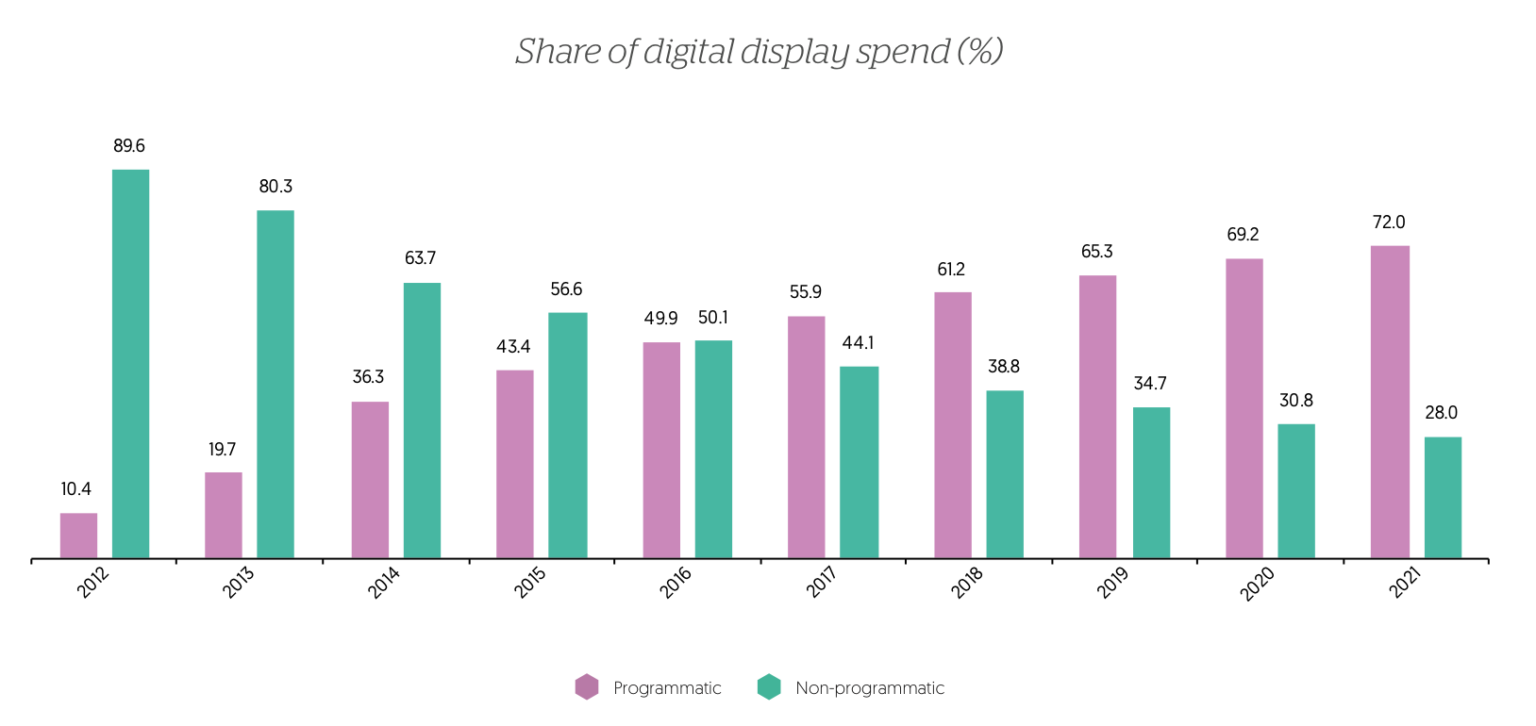
\includegraphics[width=\textwidth]{share-of-programmatic}
\centering
\end{figure}

Одной из причин столь активного вытеснения старых подхов стало повышение эффективности алгоритмов таргетинга. 

В данный момент таргетированная реклама одна из наиболее развивающихся областей digital-рекламы, так как позволяет максимально гибко и точно задать необходимую целевую аудиторию для каждого рекламного объявления. Существует ряд компаний, предоставляющих услуги по размещению таргетированной рекламы в своих рекламных сетях. Но все они имеют такие существенные недостатки как отсутствие прямого доступа к целевой аудитории, а также строгая зависимость от условий, устанавливаемых рекламными площадками. Все это создает трудности в воплощении нестандартных подходов для компаний, которые по каким-либо причинам не могут выполнить установленные требования и дает все основания задуматься о создании собственной рекламной сети.

Компания Fulldive разработала приложение Fulldive VR, которое входит в топ-5 приложений для Android в категории VR. Fulldive Browser - второй и активно развивающийся продукт компании. Одной из его наиболее важных и эффективно влияющих на привлечение новых пользователей возможностью является возможность пользователя монетизировать свое время, проведенное за чтением новостей, общением в социальных сетях, просмотром роликов и другими действиями типичными для любого другого браузера. Достигается это за счет того, что компания отдает пользователю часть прибыли, полученной от рекламных сетей за просмотры рекламы, совершенные данным пользователем в нашем приложении. 

Далеко не все рекламные площадки приветствуют такой способ мотивации пользователей, но реализация рекламы внутри своих приложений с использованием собственной рекламной сети поможет избежать данной проблемы. Это позволит компании в полной мере следовать своей стратегии развития не боясь сокращения или потери доходов от рекламы в будущем, а также позволит не отдавать часть прибыли сторонним рекламным площадкам.

Таким образом, можно выделить следующие преимущества наличия у компании собственной рекламной сети:

\begin{enumerate}
	\item Диверсификация риска сокращения прибыли от рекламы из-за прекращения сотрудничества с основными рекламными сетями
	\item Возможность добавления собственных рекламных форматов
	\item Возможность более тонко настраивать где и в каком контексте будет показана реклама
	\item Возможность сбора данных непосредственного взаимодействия пользователей с рекламой (First-Party Data), которые представляет наивысшую ценность, так как является наиболее точными, качественными и принадлежат компании
	\item Возможность использования собственной рекламной сети для привлечения сторонних рекламодателей
\end{enumerate}

Целью данной работы является создание собственной рекламной сети \textbf{UniAds}, для функционирования которой необходимо разработать соответствующее программное обеспечение.

В первой главе рассмотрен вопрос…

В второй главе рассмотрен вопрос…

В третьей главе рассмотрен вопрос…

Заключение ...

%{\large О компании Fulldive}
%\\
%Успех VR приложения и, как следствие, появление идеи развития браузера
%\bigbreak

%{\large Идеология браузера:}
%\begin{itemize}
%	\item убирать всю рекламу на сайтах
%	\item вместо нее показывать собственную рекламу
%	\item прибыль полученную за публикацию своей рекламы делить с пользователями пополам
%\end{itemize}
%\bigbreak

%{\large Плюсы:}
%\begin{itemize}
%	\item "органическое" привлечение пользователей, желающих монетизировать свое времяпрепровождении в интернете
%	\item у наших пользователей появляется возможность монетизировать свое время, проведенное в интернете (данный вид заработка особенно актуален в странах с низким уровнем доходов и занятости населения. Молодые люди, проходящие обучение в средних или высших учебных заведениях, так или иначе использующие интернет в своих образовательных и развлекательных целях, теперь могут еще и получать за это деньги. Более того, подобный способ получение дохода как никогда актуален в текущий период мирового экономического кризиса, массового сокращения рабочих мест и увеличение доли малообеспеченного населения).
%\end{itemize}
%\bigbreak

%{\large Минусы:}
%\begin{itemize}
%	\item крупные рекламные площадки либо не одобряют такую схему разделения доходов, либо пока относятся к этому индифферентно
%\end{itemize}
%\bigbreak

%(большая аудитория VR приложения (в каких странах пользуются?) -> (гипотеза) ожидается рост аудитории браузера (желательно сроки и цифры, хотя бы примерно) в таких-то странах (список на основе статистики использования Browser / VR (так как можно перелить часть аудитории в браузер)) -> (гипотеза) в этих странах локальные рекламодатели, которые захотят получить доступ к нашей аудитории? (нужна ли она им? скорее всего да, если довольно большая) -> (гипотеза) используют нашу рекламную сеть (какие есть конкуренты? почему они должны выбрать именно нас?)
%\bigbreak




%% Начало содержательной части.




\chapter{Обзор предметной области}\label{chapter:1}


\startrelatedwork %% Так помечается начало обзора.

\begin{quotation}
  Описание того как на данный момент устроены рекламные платформы, термины и общая структура
\end{quotation}

Задачи и цели таргетированной рекламы
Как и любой другой канал коммуникации с пользователями, таргет преследует несколько целей: информирование юзеров о бренде или продукте, продажа товара, привлечение внимания, обучение потребителей.

Эксперты СММ выделяют несколько видов задач, которые решает таргет:

Сбор целевых посетителей, которые интересуются продуктом или услугой и готовы покупать.
Быстрое донесение информации о продукте, бренде, акциях до ЦА и побуждение посетителей перейти на источник для подробного ознакомления.
Совершение целевого действия на месте – покупка, заявка, подписка, регистрация и другое.
Принцип работы
В основе технологии таргетинговой рекламы лежит принцип получения наиболее полной информации о пользователе. Далее система обрабатывает массив данных, сегментируют посетителей по категориям в соответствии с метриками. В соцсетях этот принцип реализуется максимально просто, так как при регистрации пользователи добровольно вводят личные данные в поля анкеты.

Например, Вконтакте предлагает заполнить такие поля: пол, возраст, день рождения, любимые фильмы, семейное положение, интересы и другие. Вся информация потом используется в таргетированной рекламе и не только.

Объявления после модерации показываются целевой аудитории, согласно настройкам кампании.

	



Провести анализ предметной области на основе первоначальных требований: существуют ли готовые решения или отдельные компоненты.
В данной предметной области достаточно много различных терминов, поэтому определим их прежде чем сформулируем подробную цель работы.

\section{Используемые термины и понятия}\label{sec:terms}

\textbf{Рекламная сеть (Ad Network)}

An advertising buying network is an online platform that acts as an intermediary between advertisers and publishers. It collects the publisher's inventory and matches it with demand coming from advertisers. Ad networks are able to sort inventory into categories according to the specific audience segments.

Целевая рекламная сеть (targeted ad network) работает точно. Наиболее продвинутый вид сетей, в связи с чем их также называют сетями 2.0. Такие сети специализируются на технологиях точного таргетирования по поведенческим или контекстным признакам, активно анализируют данные о пользователях в целях повышения стоимости инвентаря, который они продают

Дополнительно описание берем отсюда https://smartyads.com/blog/create-your-own-ad-network/

Примеры рекламных сетей: Facebook, Google AdMob, ...

\textbf{Основные роли в рекламной сети}

Рекламодатель (Advertiser)

Рекламодатель как пользователь рекламной сети:
создает рекламные материалы различных форматов (ad format) = "типов инвентаря" (inventory type) рекламной сети
конфигурирует (таргетирует) аудиторию для данного рекламного материала
указывает белый / черный список возможных плейсментов (отдельные площадки или категории площадок, отдельные разделы конкретных площадок, …)

Издатель (Publisher)

Publisher как пользователь рекламной сети:
создает (регистрирует) плейсменты доступных "типов инвентаря" рекламной сети, указывает параметры площадки: тематику, тип и объем доступной ему аудитории и т.д.
указывает белый / черный список возможных рекламодателей / рекламных агенств (отдельные или по категориям)

Advertisers don't know which websites serve their ads. Publishers don't know what companies buy their inventory.

\textbf{DSP / SSP ?}

\textbf{Ad server}

 Рекламный сервер (англ. Ad Server) \cite{ad-server}

Существует два типа рекламных серверов: один — для рекламодателей, другой — для издателей (рекламных площадок). Их отличие заключается в организации данных и удобстве работы для каждой группы пользователей.

Рекламодатели используют единый сервер объявлений, где хранится рекламный контент и предоставляется функционал для отчетов по показам, кликам и другим метрикам. Такой централизованный сервис, контролирующий распространение контента на сайтах, делает удобным отслеживание и управление рекламными материалами, повышает точность таргетинга.

Издатели — владельцы площадок — имеют отдельные рекламные серверы (только для своих доменов). Это удобно, поскольку у них есть доступ только к тому рекламному контенту, который требуется для публикации, и не нужно фильтровать все рекламные материалы на централизованном сервере.

\textbf{Таргетинг}

Решение о показе того или иного рекламного объявления принимается на основе следующей информации:
\begin{itemize}
	\item контекста плейсмента (inventory placement) для рекламы (Content and contextual targeting \cite{contextual-targeting}),
	\item накопленных данных о пользователе (Behavioral targeting \cite{behavioural-targeting}): страна, соц-дем, устройства, категории интереса (подробнее это все расписано в TargetingOptions) 
\end{itemize}

Targeting Options \url{https://adprofs.co/how-to-evaluate-demand-side-platform-companies/#targeting}

\textbf{Трекинг}
Tracking data: Track / Impression / Click / Sell
Основная воронка трекинга, open vs closed funnels

\textbf{Метрики и показатели}
CTR
CPA (CPI, CPS)
OpenRate = fill rate

\begin{quotation}
  Сайт = рекламная площадка (в нашем случае это мобильное приложение)
\end{quotation}

\section{Основной бизнес-процесс}

стадия 0: поиск и интеграция исходных рекламодателей
\\
результат 0: исходные рекламодатели (Amazon, EBay, Aliexpress, ...)
\\
стадия 1: фильтрация товаров и обогащение сторонними данными (отзывы, локализация, …)
\\
результат 1: рекламные объявления UniAds или рекламные провайдеры: UniAds, Facebook, Google AdMob, …
\\
стадия 2: фильтрация и ранжирование уже созданных объявлений
\\
результат 2: показы объявлений
\\
стадия 3:
\\
результат 3: переходы (клики)
\\
стадия 4:
\\
результат 4: конверсии (продажи, установки приложения, …)
\\
стадия 5: выделение конверсий с максимальной возможной прибылью
\\
результат 5: прибыль
\\	

\section{Постановка задачи}

Для достижения поставленной цели необходимо решить основную задачу, которая заключается в разработке программного обеспечения, необходимого для полноценного функционирования рекламной сети.

Для удобства и простоты дальнейшего описания подзадач, под аббревиатурой ПО будем понимать программное обеспечение, необходимое для решение основной задачи.

Для полноценного выполнения поставленной задачи необходимо решение следующих подзадач:
\begin{itemize}
\item разработка контракта клиент-серверного взаимодействия
\item выделение списка необходимых моделей 
\end{itemize}



\section{Требования}\label{sec:requirements}


\textbf{Общие базовые (Бизнес-требования)}
\begin{itemize}
	\item Возможность показывать товары с Amazon в виде рекламных объявлений
	\item Компания Fulldive единственный Publisher и единственный Advertiser (в будущем могут быть и другие рекламодатели)
	\item Модели ценообразования CPC и CPM (другие не поддерживаем)
	\item возможность создания и получения единичных объявлений
	\item возможность получения списка рекламных объявлений для показа на одной странице
	\item глобальный Postback для учета конверсий: покупок, установок приложения и т.д. (нужен только для модели CPA: CPI, CPS, …)
	\item трекинг данных статистики показов, переходов и пр. каждого рекламного объявления
	\item сбор данных по данным трекинга
\end{itemize}

\textbf{Требования к показу единичных объявлений:}
\begin{itemize}
	\item возможность задания категории объявления
	\item возможность задания списка стран, в которых будет показано объявление
\end{itemize}

\textbf{Требования к показу списка объявлений:}
\begin{itemize}
	\item консистентность списка для пользователя / конкретного девайса пользователя
	\item возможность фильтрации провайдеров / товаров?
	\item возможность учета для каждого товара из списка: показов и кликов
\end{itemize}

\textbf{Требования к форматам рекламных объявлений}
\begin{itemize}
	\item поддержка нативного формата (изображения с различными разрешениями + текст)
	\item поддержка баннерного формата (HTML разметка)
	\item поддержка видеоформата
\end{itemize}

\textbf{Требования к аналитике:}
\begin{itemize}
	\item возможность просмотра статистики каждого рекламного объявления в формате (AdId, Показы, Клики, CTR, тут колонки таблицы) с фильтрацией по … и группировкой по …
	\item возможность просмотра параметров эффективности (OR, CTR) стратегий таргетинга, рассчитанных по данным трекинга, с фильтрацией по интервалу дат и группировкой по идентификатору стратегии
\end{itemize}

\textbf{Технические требования:} 

Пиковая нагрузка

количественные параметры (количество показов, кликов в секунду / сутки, максимальное количество ошибок за сутки / месяц)
время ответа на 95 процентиле (P95) не более 200 мс

Стандартная нагрузка ...

\textbf{Общие сценарии использования}
\begin{itemize}
	\item Издатель запрашивает одно рекламное объявление
	\item Издатель запрашивает список рекламных объявлений
\end{itemize}

\section{Обзор существующих решений}

\begin{itemize}
\item Revive Adserver (Open-source, PHP)
\item AdGlare Ad Server (Платный)
\item Adzerk
\item AdButler
\end{itemize}


\finishrelatedwork %% Так помечается конец обзора.


\chapterconclusion







\chapter{Описание предложенного решения}\label{chapter:2}

В данной главе . Описываются основные компоненты рекламной сети, клиент-серверное взаимодействие, модели и сценарии использования.

В ходе данной работы необходимо реализовать Ad Server (единственный для рекламодателя и издателя). Результат в виде JSON API с авторизацией

\section{Клиент-серверное взаимодействие}

Взаимодействие клиента и сервера происходит по заранее установленному контракту, реализованному поверх HTTP протокола и представляет из себя несколько сценариев, которые будут подробнее описаны далее.

Разделение функций между клиентом и сервером происходит по модели распределенного представления данных.

\begin{figure}[h]
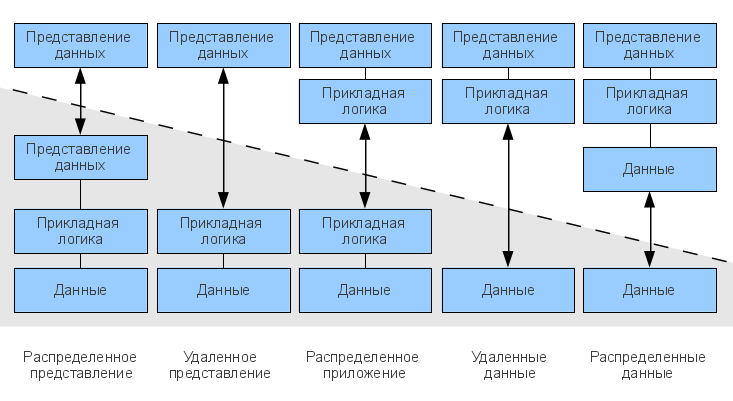
\includegraphics[width=\textwidth]{cs-models}
\centering
\end{figure}

Cервер отвечает за управление рекламным инвентарем и объявлениями, сбор статистики показов, переходов и конверсий, поддержание внутренних инвариантов для сохранения актуальности и консистентности данных. Клиент отвечает за корректное отображение полученных от сервера рекламных материалов.

\section{Трёхуровневая архитектура}

В качестве архитектуры серверного приложения используется трёхуровневая архитектура (англ. three-tier architecture) \cite{three-tier-architecture}, в которой разделяются функции представления, обработки и хранения данных. Разделяя приложение на уровни абстракции, появляется возможность внесения изменений в какой-то определённый слой, вместо того, чтобы перерабатывать всё приложение целиком. Трёхуровневая архитектура обычно состоит из слоя представления, слоя бизнес-логики и слоя хранения данных.

(тут картинка со слоями)

Перед тем как приступить к детальному описанию выбранной архитектуры перечислим основные модели, которые представляют объекты предметной области, а затем последовательно рассмотрим каждый из слоев абстракции серверного приложения. 

\section{Модели}\label{sec:models}

\subsection{AdProvider}
Только Amazon

\subsection{Ad}

Модель Ad состоит из следующих полей:
\begin{itemize}
\item уникальный идентификатор объявления
\item идентификатор продукта
\item тип объявления 
\item контент объявления, представленный ссылками на изображения и видео, используемыми для отображения объявления на клиенте
\item ссылка для перехода по нажатию
\item идентификатор провайдера объявления
\item цена
\item категория
\end{itemize}

\subsection{StrategyState}

Модель StrategyState состоит из следующих полей:
\begin{itemize}
\item идентификатор стратегии (одна из стратегий, описанных в \ref{sec:strategies})
\item идентификтор потока (thread в \ref{sec:strategies-state})
\item номер версии
\item набор пар (идентификатор объявления, скоринг объявления)
\end{itemize}


\subsection{Session}
...

\subsection{Track, Impression, Click}
...

\section{Слой хранения данных}

Слой данных (англ. data access layer) \cite{data-access-layer} состоит из репозиториев. Репозиторий (англ. repository pattern) \cite{repository-pattern} обеспечивает абстракцию данных таким образом, что приложение может работать с простой абстракцией, интерфейс которой приближен к интерфейсу коллекции. 

Добавление, удаление, обновление и получение элементов из этой коллекции выполняется с помощью ряда простых методов без необходимости решать проблемы с базами данных, такие как соединения, команды, курсоры. Использование этого шаблона позволяет добиться слабой связности и отсутствию зависимости от способа хранения данных. Таким образом вся логика необходимая для функционирования моделей содержится в репозиториях.

Исходя из представленных моделей \ref{sec:models} и требований к рекламному серверу \ref{sec:requirements} репозитории делятся на три группы:
\begin{itemize}
\item репозитории сущностей рекламных объявлений
\item репозитории сущностей, используемых в таргетинге
\item рапозитории сущностей, используемых в трекинге
\end{itemize}

TODO Кратко описываем интерфесы для каждой группы репозиториев (Ad, Targeting, Tracking) и кэша (AdCache)

\section{Слой бизнес-логики}

Модуль - это высокоуровневые элементы - Service, Job. Компоненты предоставляющие доступ к хранилищам моделей будут привежены в 3-й главе.

Далее рассмотрим слой логики с разбиением на модули.

\begin{figure}[h]

\includegraphics[width=\textwidth]{placeholder}
\centering
\end{figure}

\subsection{Обновление объявлений}

Обновление рекламный объявлений является автоматическим и в контексте нашего сервиса выполняет функцию рекламодателя. Стадии данного процеса описываются следующим алгоритмом:
\begin{enumerate}
\item отбор актуальных товаров на Amazon по заранее заданным критериям
\item генерация рекламных объявлений на основе полученных товаров
\item сохранение полученных объявлений в базе данных
\item деактивация уже существующих в системе объявлений и активация только что созданных
\end{enumerate}

\begin{figure}[h]

\includegraphics[width=\textwidth]{placeholder}
\centering
\end{figure}

\subsection{Кэширование объявлений}

Актуальность кэша рекламных объявлений необходима, т.к. кэш является источником истины объявлений в стратегиях таргетирования (показать на схеме?)

\subsection{Обновление категорий интереса пользователя}

По просмотренным страницам 

По кликам на рекламные объявления


\subsection{Таргетинг}

Таргетинг = ранжирование (относительные величины - порядковые номера)/ скоринг (абсолютные величины) + эвристики фильтрации + небольшая рандомизация (в будущем можно сделать на основе TargetingOptions (для этого можно использовать сторонее решение? какое?)

Каждая стратегия таргетирования назначает веса рекламным объявлениям \ref{creative-sequencing}, чтобы управлять их частотой показа. Три группы объявлений (нарисовать автомат переходов): testing, rejected, approved. Рандомизация применяется для равномерного показа объявлений внутри своей группы. 

\textbf{Выбор оптимальной стратегии} на основе данных, представленных в запросе (A/B тестирование стратегий): если рекламное объявление должно зависеть от контекста, в котором оно будет показано выбирается одна из стратегий, которая таргетирует на основании параметров переданного контекста. Иначе выбирается стратегия, которая таргетирует на основании накопленных знаниях о категориях интереса текущего пользователя.

(почему именно так решать?)

\subsection{Стратегии таргетинга}\label{sec:strategies}

\textbf{Для таргетирования используются 4 стратегии}:
\begin{enumerate}
	\item случайные объявления
	\item объявления с глобально высоким показателем CTR
	\item объявления с высоким показателем CTR в категориях интереса данного пользователя, рассчитанных на основе просмотренных страниц в интернете
	\item объявления с высоким показателем CTR в категориях интереса данного пользователя, рассчитанных на основе кликов по объявлениям внутри приложения
\end{enumerate}

Расписать принцип работы каждой из 4-х стратегий: матчинг категорий - random (стратегия создавалась для быстрого получения MVP), по кликам overall, по просмотрам страниц (IBM Watson NLP), по кликам на объявления (Категории товаров Amazon)

\subsection{Состояния стратегий}\label{sec:strategies-state}

\textbf{StrategyState threads} (обновление состояний потока по расписанию (а также при запросе?))

\textbf{StrategyState resolving} (N.B. sessionKey по идее может быть произвольной строкой предоставляемой Publisher'ом) Использует структурный шаблон проектирования Flyweight для уменьшения потребления оперативной памяти для хранения большого сессий.

\begin{figure}[h]

\includegraphics[width=\textwidth]{placeholder}
\centering
\end{figure}

\subsection{Трекинг показов и переходов}

Трекинговая закрытая воронка (Track / Impression / Click / Sell)

\begin{figure}[h]

\includegraphics[width=\textwidth]{placeholder}
\centering
\end{figure}

\textbf{Сценарии использования накопленных данных трекинга (ответ на вопрос: для чего мы собираем эти данные?):}
\begin{itemize}
	\item (ручное использование) расчет (real-time?) статистики по рекламным объявлениям: Impressions, Clicks, Conversions? (в основном для сторонних рекламодателей), CTR, CR для отображение в панели рекламодателя
	\item (автоматическое использование) использование CTR рекламного объявления в стратегиях таргетирования (Global Interesting Strategy, Interesting in Category Strategy, …)
	\item (ручное использование) оптимизация бизнес процесса на основе данных (Data-driven decision making)
	\item  (автоматическое использование) автоматический выбор стратегии таргетирования на основе статистики стратегий
\end{itemize}


\subsection{Актуализация рекламного инвентаря}

Издатель запрашивает актуальный рекламный инвентарь на сервере конфигурации и сохраняет его в базе данных.

\begin{figure}[h]

\includegraphics[width=\textwidth]{placeholder}
\centering
\end{figure}

\section{Сценарии использования}

Слой клиента представляет из себя контракт взаимодействия клиента и сервера

Получение данных клиентом подразумевает отправку HTTP запросов  на сервер в установленном формате и с токеном для подтверждения доступа.

Далее рассмотрим совместное функционирование приведенных модулей в основных сценариях использования.
Два типа триггеров - запрос к серверу, запуск по расписанию в контексте задачи.

\subsection{Получение одного объявления}
Получение данных пользователя. 
Выбор стратегии таргетинга. 
Получение списка объявлений по выбранной стратегии.

\subsection{Получение списка объявлений}
Получение данных пользователя и текущей сессии (у каждой сессии свой уникальный ключ). 
Выбор стратегии таргетинга. 
Получение списка объявлений по выбранной стратегии.

\subsection{Трекинг показов и переходов}
...

\subsection{Получение статистики по стратегиям таргетинга}
...

\chapterconclusion

Вывод в конце второй главы






\chapter{Техническая реализация и внедрение предложенной архитектуры}

Здесь описывается итоговая архитектура рекламной сети (инфраструктура, количество серверов, тип масштабирования, базы данных, кэширование...

Описываем текущую инфраструктуру компании: Kubernetes кластер, микросервисы общаются по AMQP.

Наш сервис -  еще один "микросервис" (почему?)

Используем платформу Node.js (почему?)

Используем язык программирования Typescript \cite{typescript-lang} версии 3.8. Основные преимущества данного языка:
\begin{itemize}
\item широко используется в различных проектах компании (уменьшает порог вхождения членов команды)
\item современный язык, разработанный компанией Microsoft (гарантирует надежность и развитие языка)
\item обладает возможностью писать как в императивном стиле так и декларативном (позволяет повысить читаемость кода и использовать функциональный стиль программирования)
\item обладает строгой типизацией (позволяет существенно сократить вероятность появления дефектов в процессе разработки и сопровождения кода)
\end{itemize}


\section{Процесс разработки}

Процесс разработки состоит из следующих стадий (переписать в контексте Agile):
\begin{itemize}
	\item сформировать требования к ПО
	\item спроектировать архитектуру ПО
	\item реализовать ПО на основе требований и модели архитектуры
	\item протестировать итоговое ПО
	\item внедрить ПО
\end{itemize}

Готовые модули, используемые в проекта, находятся в реестре публичных Node.js модулей - NPM (ссылка)

Используем Git (git-flow / GitHub-flow), Bitbucket (pull-requests, code-review)

\section{Инфраструктура}

Описать что такое кластер в Google Kubernetes Engine

\subsection{Хранение изображений}
Хранение изображений в Google Buckets. Также работает как CDN

\section{Конфигурация, окружение}

Множество окружений: staging, production \cite{twelve-factor-app}


\section{Аутентификация запросов}

Аутентификация: JWT


\section{Работа с моделями}

\subsection{Модель Ad}

Модель Ad состоит из сущностей Ad, AdMedia, Price (отношения one-to-many). Для хранения этих сущностей используется база данных MongoDB \cite{mongodb} (почему? т.к. база общего назначение + является основной в компании, позволяет относительно безболезненно вносить изменения в схему данных)

\subsection{Модели трекинга}

Track, Impression, Click (ClickHouse, т.к. нужна поддержка OLAP)

\subsection{ORM}

Выбор ORM и драйверов для работы с БД: какие выбраны и почему?



\section{Обновление объявлений (AdUpdater)}

Так как объявления формируются на основе товаров с Amazon, то для начала нам надо определиться какие именно товары мы хотим показывать нашим пользователям.

\subsection{Критерии отбора товаров}

\subsection{Получение товаров через Product Advertising API}

На данный момент официальным и актуальным способов доступа к товарам, размещаемым на площадке Amazon является интерфейс Product Advertising API 5.0 \cite{amazon-paapi-docs}. Доступ к API осуществляется с помощью access-token. Соединение происходит по HTTP протоколу, формат запросов и ответов - JSON. Для осуществеления авторизованных запросов используется Node.js SDK \cite{amazon-paapi-sdk}

В ссылку на товар подставляется \textit{PartnerTag} для связывания покупок, совершаемых по данной ссылке, с партнером, который привел покупателя.

\subsection{Создание объявления}

Как мы расфасовываем Resource по сущностям Ad, AdMedia, Price.

\textbf{Обновление Price}

Заменяем текущее значение модели Price связанной с Ad на новое

\textbf{Обновление AdMedia}

При обновлении Ad уникализируем связанные с ним AdMedia по url, чтобы не плодить кучу копий со статусом enabled = false в базе.


Оборачивание ссылки с помощью RedirectEncoder для отслежвания переходов. (переместить в контроллер!)



\section{Кэширование объявлений (AdService + AdCache)}

Обновление объявлений, описанное в предыдушей подглаве, инициирует обновления кэша объявлений для сохранения консистентности. Это важно так как 
Кэш объявлений и скоринга. Redis, т.к. нужен быстрый доступ к объявлениям) . Обосновать выбор той или иной базы для каждой сущности, желательно найти бенчмарки сравнения MongoDB и Redis)

\section{Обновление состояний стратегий (StrategyStateUpdater)}

Каждое состояние рассчитывается и сохраняется для последующих обращений в Redis , так как расчитывать весь список объявлений на каждый запрос к существенному увеличению времени ответа, а также абсолютно чрезмерному и неоправданному использованию серверных мощностей.

(Amazon <-> IBM Watson category mapper)

\section{Контроллеры}

Для обработки запросов, поступающих к нашему микросервису, используется фреймворк Koa2 (ссылка), работающий поверх веб-сервера Node.js (ссылка).

Контроллер реализуется посредством использования класса "middleware" (который является примером поведенческого паттерна проектирование Chain of Responsibility)

Список контроллеров, по каждому входные параметры и выходные параметры (объемные ответы в виде ссылок на примечание)

\section{Документация}

Документация openapi.yml


\section{Тестирование}

\subsection{Концепция написания тестов}

Процесс тестирования полученной платформы: Unit/Integration/Functional/E2E тестирование, White-box/Black-box, в каком количестве? для проверки чего и какие виды тестов использовались?

Вставки с кодом тестов для иллюстрации фреймфорка: сетап-действие-ассерт (https://bitbucket.org/fulldivevr/community-doc/src/master/tdd-conspect.md)

\subsection{Локальное тестирование}

Как производится локальное тестирование не-unit тестов: Docker, docker-compose

Команды для запуска тестирования в package.json: test:unit, test:e2e и т.д. (mocha, chai)

\section{Внедрение}

Процесс внедрения (развертывания): , описание *.yaml файлов конфигурации, helm-charts, skaffold; BitBucket pipelines; Terraform; тэги и версионирование

\chapterconclusion

Вывод в конце третьей главы





%% Макрос для заключения. Совместим со старым стилевиком.
\startconclusionpage

Дальнейшее развитие (стратегические направления / цели) (исходя из них можно уточнить требования к реализации платформ
(все дальнейшие разработки и улучшения также направлены на увеличение прибыли (согласно основному бизнес-процессу итоговая цель - прибыль))

N1 Развитие компании в качестве своего собственного рекламодателя (growth as Advertiser / Ad provider). Как это сделать?
\begin{itemize}
\item Идея 1: увеличить количество исходных рекламодателей - интегрировать E-commerce платформы Ebay, Aliexpress, Wildberries, …
\item Идея 2: подбирать множество товаров таким образом, чтобы итоговое число покупок было максимально (слишком мало товаров - неудовлетворенный спрос, слишком много товаров - проблема выбора и рассеивание внимания)
\item Идея 3: тиражирование товаров с максимально высокой вероятностью покупки для конкретного пользователя, например, товары из интересующих пользователя категорий (персонализация показываемой рекламы)
\end{itemize}

N2 Оптимизация количества и качества плейсментов внтури приложений компании (growth as Publisher)

N3 Привлечение сторонних рекламодателей (добавление RTB / Bidders)

\printmainbibliography

%% После этой команды chapter будет генерировать приложения, нумерованные русскими буквами.

\appendix

\chapter{Графики}\label{sec:app:1}

графики отсюда https://www.smartinsights.com/internet-advertising/internet-advertising-targeting/what-is-programmatic-marketing/

\chapter{Примеры ответов на запросы}\label{sec:app:2}

примеры запросов и ответов API (ad, ads)

\chapter{Категории товаров на Amazon}\label{sec:app:3}

(список категорий)

\chapter{Картинки из Android приложения}\label{sec:app:4}

скрины одиночных объявлений (лента, страница) + products feed

\end{document}